\documentclass[12pt,xcolor=svgnames]{beamer}
\usepackage{dsfont,natbib,setspace,changepage}
\mode<presentation>

% fonts
\usepackage{pbsi}
\usefonttheme[onlymath]{serif}

% replaces beamer foot with simple page number
\setbeamertemplate{navigation symbols}{}
\setbeamertemplate{footline}{
  \raisebox{10pt}{\makebox[\paperwidth]{\hfill\makebox[20pt]{\color{gray}\scriptsize\insertpagenumber}}}}

% color 
\newcommand{\bk}{\color{black}}
\newcommand{\rd}{\color{red}}
\newcommand{\fg}{\color{ForestGreen}}
\newcommand{\bl}{\color{blue}}
\newcommand{\gr}{\color{gray}}
\newcommand{\sg}{\color{DarkSlateGray}}
\newcommand{\nv}{\color{Navy}}

\newcommand{\theme}{\color{Maroon}}
\graphicspath{{/green/Dropbox/inputs/},
{/Users/mtaddy/Dropbox/inputs/},
{/home/taddy/project/bigdata/graphs/},
{/Users/mtaddy/project/bigdata/graphs/}}

% style
\setbeamercolor{itemize item}{fg=gray}
\setbeamercolor{itemize/enumerate body}{fg=DarkSlateGray}
\setbeamercolor{frametitle}{fg=black}
\setstretch{1.1}

% common math markups
\newcommand{\bs}[1]{\boldsymbol{#1}}
\newcommand{\mc}[1]{\mathcal{#1}}
\newcommand{\mr}[1]{\mathrm{#1}}
\newcommand{\bm}[1]{\mathbf{#1}}
\newcommand{\ds}[1]{\mathds{#1}}
\newcommand{\indep}{\perp\!\!\!\perp}

% shorthand
\newcommand{\sk}{\vspace{.5cm}}
\newcommand{\R}[1]{{\tt \nv #1}}
\newcommand{\til}{{\footnotesize$\bs{\stackrel{\sim}{}}$ }}

\begin{document}

\setcounter{page}{0}
{ \usebackgroundtemplate{
\includegraphics[height=\paperheight]{phoenix}}
\begin{frame}[plain]
\begin{center}


{\bf \Large [{\large $\bs{\star}$}] Big Data: {\theme Spatiotemporal Data}}

\vskip 1.5cm 
Matt Taddy, University of Chicago Booth School of Business

\vskip .2cm 
\texttt{faculty.chicagobooth.edu/matt.taddy/teaching} 


\end{center}
\end{frame} }

\begin{frame}

{\bf \nv Space-Time data is everpresent.}

\vskip .5cm


In this class we've focused on \\independent and 
identically distributed ({\theme iid}) data.

We haven't talked much about space-time dependence.

\sk
The first-order trick with such data is de-trending:\\
Use `standard' methods to get data that should be iid.

\vskip .25cm
\begin{itemize}
\item Using returns rather than prices.
\item `seasonally adjusted': financial data is often pre-cleaned.
\item Include time {\tt+} space variables in your regression.
\end{itemize}

\vskip .25cm
This class has made the `include time variables' step trivial, since
we just throw everything in and let CV-lasso sort it out.

\end{frame}

\begin{frame}

{\bf  Spatiotemporal Trends}


\sk The data often include time $t$ {\gr (year, day, second)}\\
or space $\bm{s}=[s_1,s_2]$ {\gr (latitude, longitude)}.

\vskip .25cm
If you have $t$ or $\bm{s}$, just put them in 
the regression. 

{\nv e.g., california housing data in trees lecture.} 

\vskip .25cm {\gr You can also add quadratic versions:} 
\\ When regressing crime on
abortion and controls ({\tt 09}),\\ we included
effects for time and time$^2$: {\theme $t\beta_t + t^2\beta_{t2}$}\\ 
{\it and} interaction of these trends with all controls 
so that the effect of, say, beer consumption was  $\theme \beta_{\mr{beer}} + \beta_{\mr{beer},t}t+
\beta_{\mr{beer},t2}t^2$.

\vskip .25cm
{\gr Then use CV-lasso to only keep what matters.\\
Alternatively, if you have lots of data, just do {\tt glm}.}

\end{frame}

\begin{frame}

{\bf Seasonality}

\sk
In temporal data, we often need to account for seasonality:

\hfill {\nv cyclical month/quarter/day/etc effects.~~~~}

\vskip .25cm
For example, maybe sales are always higher in spring/summer, or beginning of quarter months are leaner than end of quarter.

\vskip .25cm 
Again, the solution is: {\theme put them in the model!}

\vskip .25cm
This time, you include seasonal indicators as dummy variables.

For example, 

\vskip .1cm
{\nv\tt\small 
~~~month = factor(month) {\theme \# levels "jan","feb",...}

~~~x = model.matrix($\sim$.+month, data=D) {\theme \# or .*month}
}

\vskip .1cm
Something like this would allow for `month effects'.


\end{frame}


\begin{frame}

{\bf Example: \theme airline data}

\sk
$Y_t = $ monthly total international airline passengers, 1949-1960.
\vskip -.5cm
~~~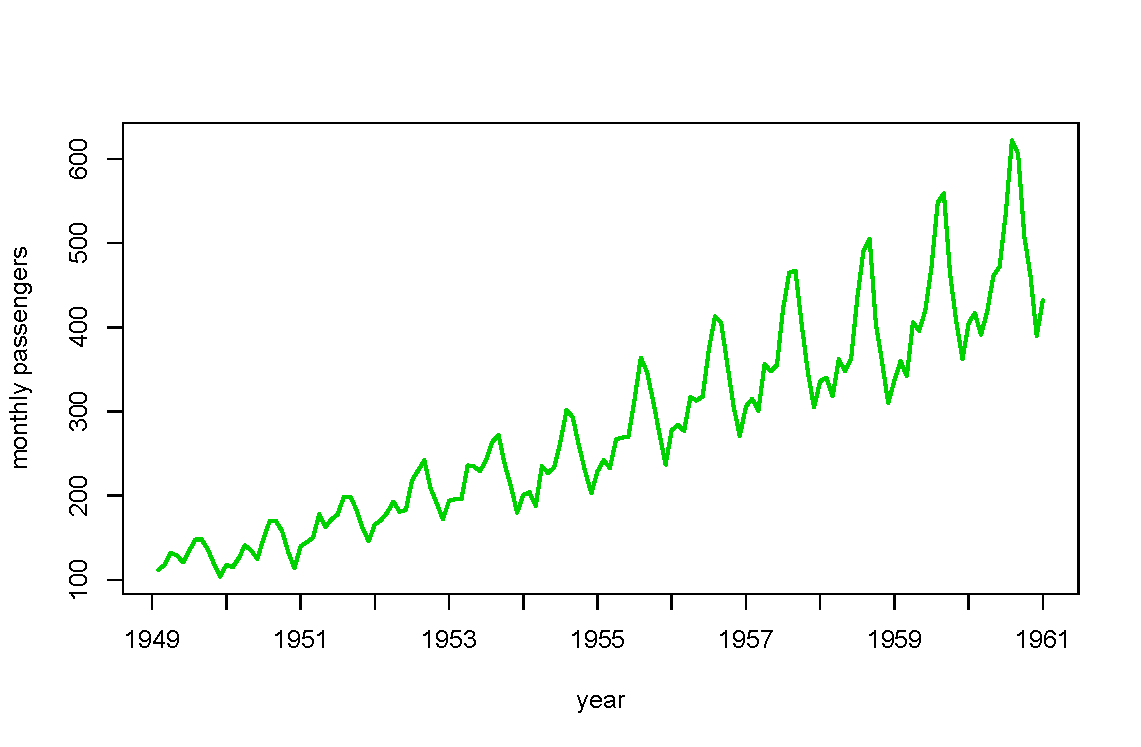
\includegraphics[width=4in]{../graphs/airline}
\vskip -.25cm
\small
We see an increasing annual oscillation and positive linear trend.

\end{frame}


\begin{frame}

{\bf Air Travel}

\vskip .25cm
Fitting the model: first, don't forget your fundamentals!
\begin{itemize}
\item The series variance is increasing in time.
\item Passenger numbers are like sales volume.
\item \theme We should be working on log scale!
\end{itemize}
\vskip -.7cm
~~~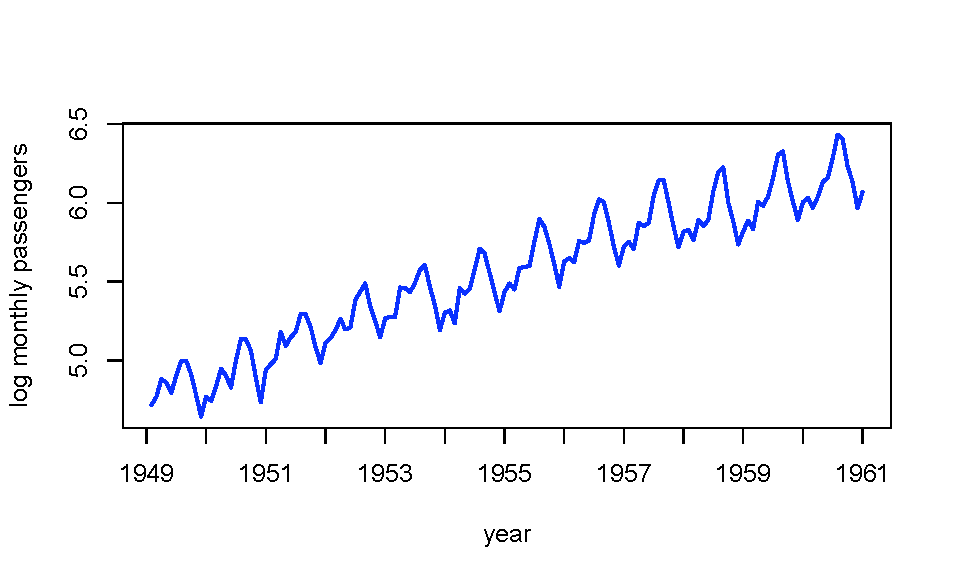
\includegraphics[width=4in]{../graphs/logairline}


\vskip -.7cm
\end{frame}


\begin{frame}[fragile]

{\bf Air Travel}

\sk
The series shows a linear trend and an oscillation of period 12

(i.e., it looks like we need month effects $\beta_{m_t}$)

\[\theme
\hskip -.5cm \log(y_t) = \alpha + \beta_tt + \beta_{m_t}
 + \varepsilon_t 
\]

\vskip -.5cm
{\nv\small
\begin{verbatim}
month <- factor(airline$Month)
time <- (year-min(year))*12 + airline$Month
summary(air <- glm(log(passengers) ~ time + month))

>               Estimate Std. Error t value Pr(>|t|)    
> time         0.0100688  0.0001193  84.399  < 2e-16 ***
> month2      -0.0220548  0.0242109  -0.911  0.36400    
> month3       0.1081723  0.0242118   4.468 1.69e-05 ***
...
\end{verbatim}}

\end{frame}

\begin{frame}


{\bf Airline Travel: model fit}

\sk
The model predictions look pretty good!

\vskip .25cm
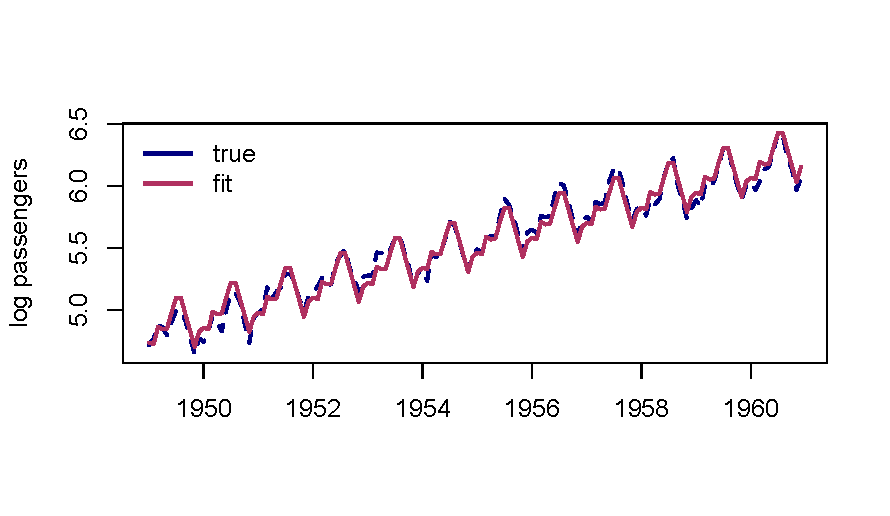
\includegraphics[width=4in]{../graphs/airlinefit}


\sk
The month and time effects seem to capture the trends.\\
{\theme However, if we look close...}

\end{frame}


\begin{frame}

{\bf Airline Travel: {\theme autocorrelation}}

\sk
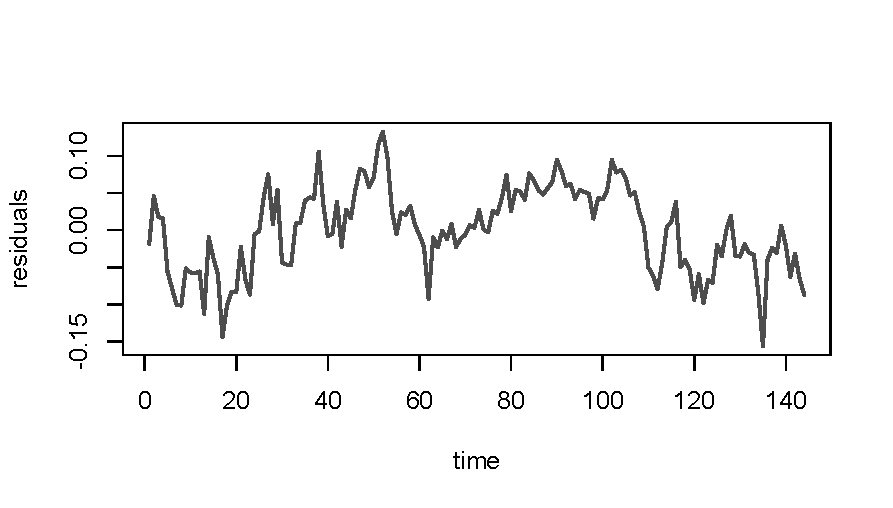
\includegraphics[width=4in]{../graphs/airlineresid}

\sk
Residuals appear correlated in time!\\
This violates our basic {iid} assumption: $\varepsilon_i \indep \varepsilon_j$.

This is called {\nv autocorrelation}: correlation with yourself.


\end{frame}

\begin{frame}

{\bf Time Series Data and Dependence}

\sk

Time-series data are simply a collection of observations
gathered over time.
For example, suppose $y_1 \ldots y_T$ are
\begin{itemize}
\item  Annual GDP.
\item  Quarterly production levels
\item  Weekly sales.
\item  Daily temperature. 
\item  5 minute Stock returns.
\end{itemize}

\sk\nv
In each case, we might expect what happens \\at time $t$ to be
correlated with time $t-1$.

\end{frame}

\begin{frame}

{\bf Time Series Data and Dependence}


\sk


Suppose we measure temperatures  daily for several  years.

\sk
Which  would work better as an estimate for today's temp:
\begin{itemize}
\item The average of the temperatures from the previous year? 
\item The temperature on the previous day? 
\end{itemize}

\sk
How would this change if the readings were iid?

\sk \theme
Correlated errors require fundamentally different techniques.

\end{frame}



\begin{frame}[fragile]

{\bf \theme The autocorrelation function}

\sk
Summarize dependence with lag-$l$ correlations:

The autocorrelation function (ACF) is
$
r(l) = \mr{cor}(\varepsilon_t, \varepsilon_{t-l})
$

\vskip .5cm

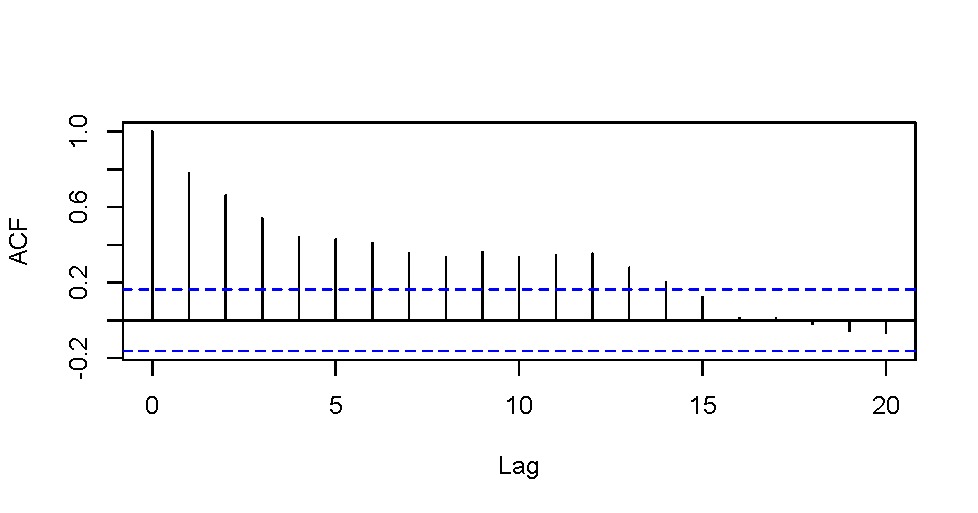
\includegraphics[width=4in]{../graphs/airlineacf}

\vskip -.25cm
{\nv \footnotesize
\begin{verbatim}
> print(acf(air$resid))
Autocorrelations of series ‘air$resid’, by lag
     0      1      2      3      4      5      6  
 1.000  0.779  0.662  0.539  0.440  0.429  0.410  
\end{verbatim}}

\vskip -.25cm

\end{frame}



\begin{frame}

{\bf Autoregression}

\sk

How do we model this type of data?

\sk Suppose $y_1 = \varepsilon_1$, $y_2 = \varepsilon_{1} +
\varepsilon_{2}$, $y_3 = \varepsilon_{1} + \varepsilon_{2} + \varepsilon_{3} +...$,

\sk
\nv
~~~~~Then $y_t =  \sum_{i=1}^{t}\varepsilon_i = y_{t-1} + \varepsilon_t$ and $\ds{E}[y_t] = y_{t-1}$.\bk

\sk
This is called a \theme Random Walk \bk model for $y_t$:  the expectation of what will happen is always what happened most recently.

\sk
Even though $y_t$ is a function of errors going all the way back to the beginning, you can
write it as depending only on $y_{t-1}$.
\end{frame}


\begin{frame}

{\bf Autoregression}
\sk

Random walks are just a version of a more general model...

\sk
The \nv autoregressive \bk model of order one holds 
\[
\theme AR(1): y_t = \beta_0 + \beta_1y_{t-1} + \varepsilon
\]
This is just an SLR model of $y_t$ regressed onto lagged $y_{t-1}$,
and it assumes all of our standard regression model conditions.

\begin{itemize}
\item The residuals should look $iid$ and be uncorrelated with $\hat{y}_t$.
\item All of our previous diagnostics and transforms still apply.
\end{itemize} 

\end{frame}


\begin{frame}

{\bf Autoregression}

{\large \[
\theme AR(1): y_t = \beta_0 + \beta_1y_{t-1} + \varepsilon
\]}
\vskip -.25cm
Again, $y_t$ depends on the past only
through $y_{t-1}$.  
\begin{itemize} 
\item[]\nv AR(1) means that previous lag values ($y_{t-2},
y_{t-3},\ldots$) \\do not help predict $y_t$ if you already know $y_{t-1}$.
\end{itemize}

\sk
Think about daily temperatures:  
\begin{itemize} \small
\item If I want to guess tomorrow's 
temperature (without knowing the forecast!), I 
base my prediction on today's temperature and will probably ignore yesterday's temperature.
\end{itemize}

\sk
{\nv In this model $\beta_1$ is called the AR term}

\end{frame}

\begin{frame}[fragile]

{\bf \theme Fitting the AR model}

{\footnotesize\nv
\begin{verbatim}
> lag <- head(log(passengers),-1)## see help(head)
> passengers <- passengers[-1]
> month <- month[-1]
> time <- time[-1]
> summary(airAR <- glm(log(passengers) ~ time + month + lag))
...
lag          0.7930716  0.0548993  14.446  < 2e-16 ***
\end{verbatim}}

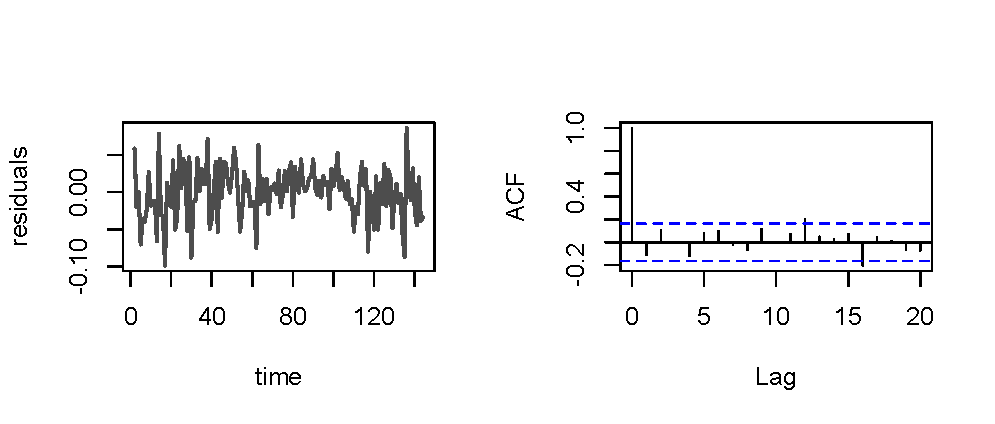
\includegraphics[width=4in]{../graphs/airlinear}

Now the residuals look nice and independent.

\end{frame}




\begin{frame}

{\bf AR(1) Autoregression}\sk

Many different types of series may be written as an AR(1).
\[
AR(1): Y_t = \beta_0 + \beta_1Y_{t-1} + \varepsilon
\]\nv
The value of $\beta_1$ is key! \bk
\begin{itemize}
\item  If $|\beta_1| = 1$, we have a random walk.
\item  If $|\beta_1| > 1$, the series explodes.
\item  If $|\beta_1| < 1$, the values are mean reverting.
\end{itemize}

\end{frame}


\begin{frame}

{\bf Random Walk}\sk

In a random walk, the series just wanders around.

\begin{center}
$\beta_1 = 1$
\end{center}
\vskip -1.5cm
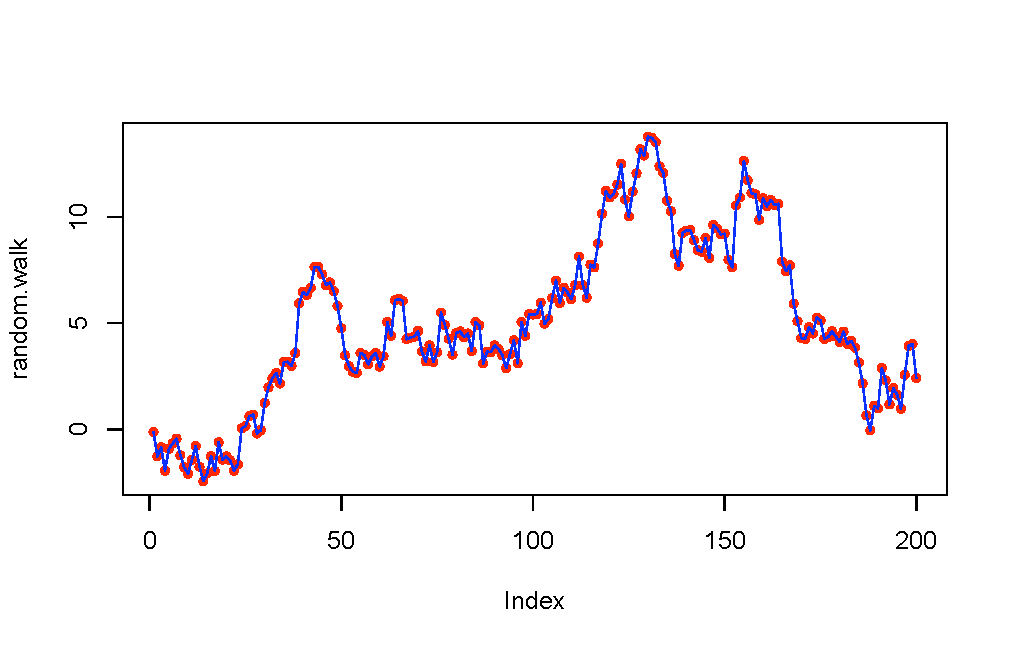
\includegraphics[width=4in]{../graphs/randwalk}

\end{frame}

\begin{frame}

{\bf Random Walk}\sk

Autocorrelation of a random walk stays high for a long time.

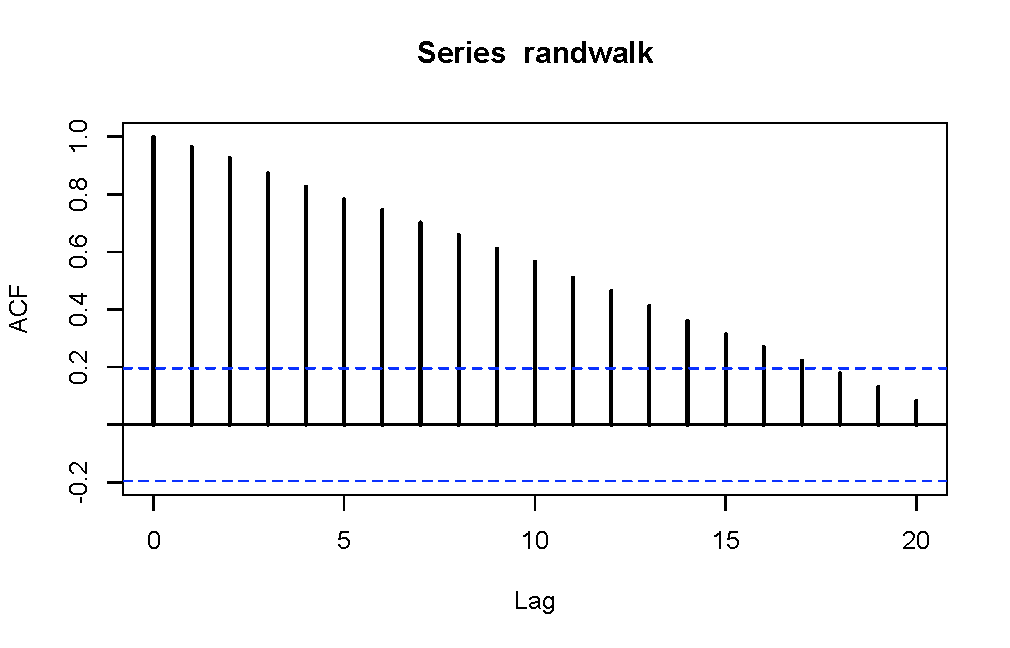
\includegraphics[width=4in]{../graphs/acfrandwalk}

\end{frame}


\begin{frame}

{\bf Random Walk}\sk

The random walk has some special properties...

\sk
$\nv Y_t - Y_{t-1} = \beta_0 + \varepsilon$, and $\beta_0$ is called the ``drift parameter''.

\sk
The series is \nv nonstationary\bk: it has no average level that it wants to be near, 
but rather just wanders off into space.

\sk Since $\nv \ds{E}[Y_t] = \ds{E}[Y_{t-1}]$ (e.g., tomorrow $\approx$
today), the random walk \theme without drift \bk is a common model for
simple processes.
\end{frame}



\begin{frame}

{\bf Random Walk Example: Dow Jones}\sk

For example, consider the monthly Dow Jones \\composite index from 2000 - 2007

\vskip -.5cm
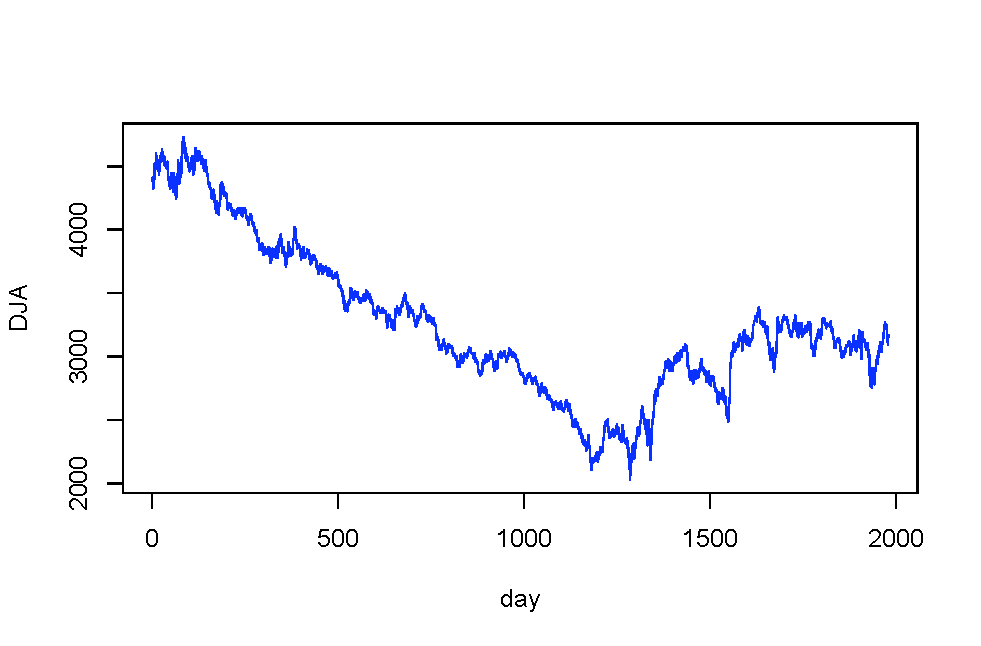
\includegraphics[width=4in]{../graphs/dja}
\vskip -.25cm
DJA appears as though it is just wandering around.
\end{frame}


\begin{frame}[fragile]

{\bf Random Walk Example: Dow Jones}\sk

\small
Sure enough, the regression fit looks like a random walk ($b_1 \approx 1$).

{\nv\footnotesize

\begin{verbatim}
> summary(ARdj <- glm(dja[2:n] ~ dja[1:(n-1)]))

...

Coefficients:
               Estimate Std. Error t value Pr(>|t|)    
(Intercept)     7.05419    4.00385   1.762   0.0782 .  
dja[1:(n - 1)]  0.99764    0.00121 824.298   <2e-16 ***
\end{verbatim}}


\end{frame}




\begin{frame}

{\bf Random Walk Example: Dow Jones}\sk

When you switch to returns, however, it's just white noise.

\vskip -.5cm
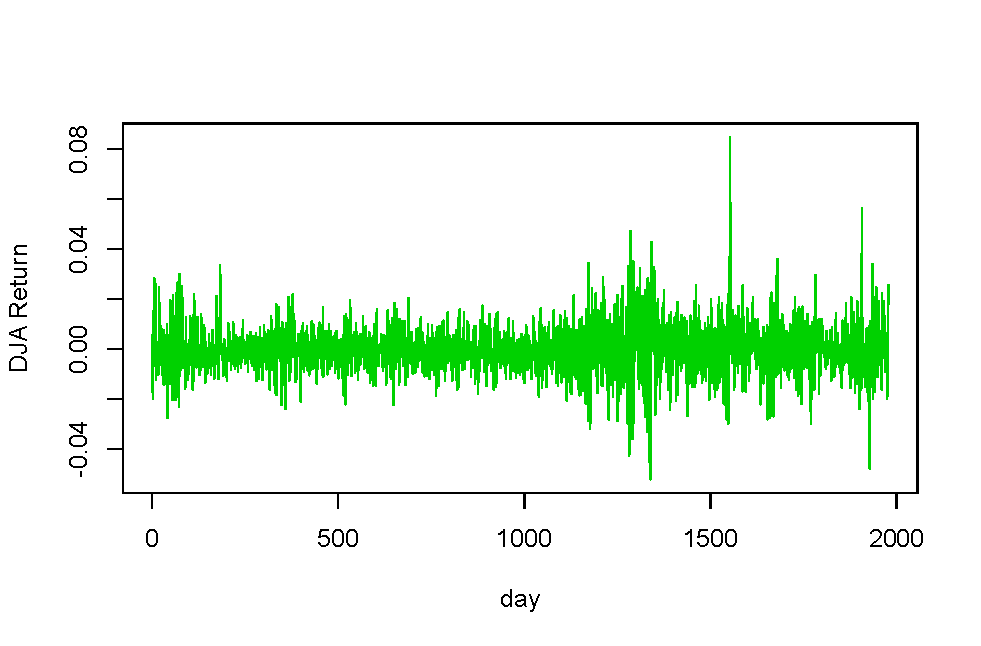
\includegraphics[width=4in]{../graphs/return}
\vskip -.25cm

$(Y_t - Y_{t-1})/Y_{t-1}$ appears to remove the dependence.

\end{frame}


\begin{frame}[fragile]

{\bf Random Walk Example: Dow Jones}\sk


And now the AR term is not significant.

{\footnotesize\nv
\begin{verbatim}
> returns <- (dja[2:n]-dja[1:(n-1)])/dja[1:(n-1)]
> summary( glm(returns[2:n] ~ returns[1:(n-1)]) )

...

Coefficients:
                     Estimate Std. Error t value Pr(>|t|)
(Intercept)        -0.0001138  0.0002363  -0.482    0.630
returns[1:(n - 1)] -0.0144411  0.0225321  -0.641    0.522
\end{verbatim}}

This is common with random walks: \theme difference  $Y_{t}- Y_{t-1}$ is iid.

\end{frame}

\begin{frame}

{\bf Exploding Series}\sk

\small For AR term $>1$, the $Y_t$ values move exponentially far from $Y_1$.

\begin{center} \vskip -.25cm
$\beta_1 = 1.02$
\end{center}
\vskip -1.5cm
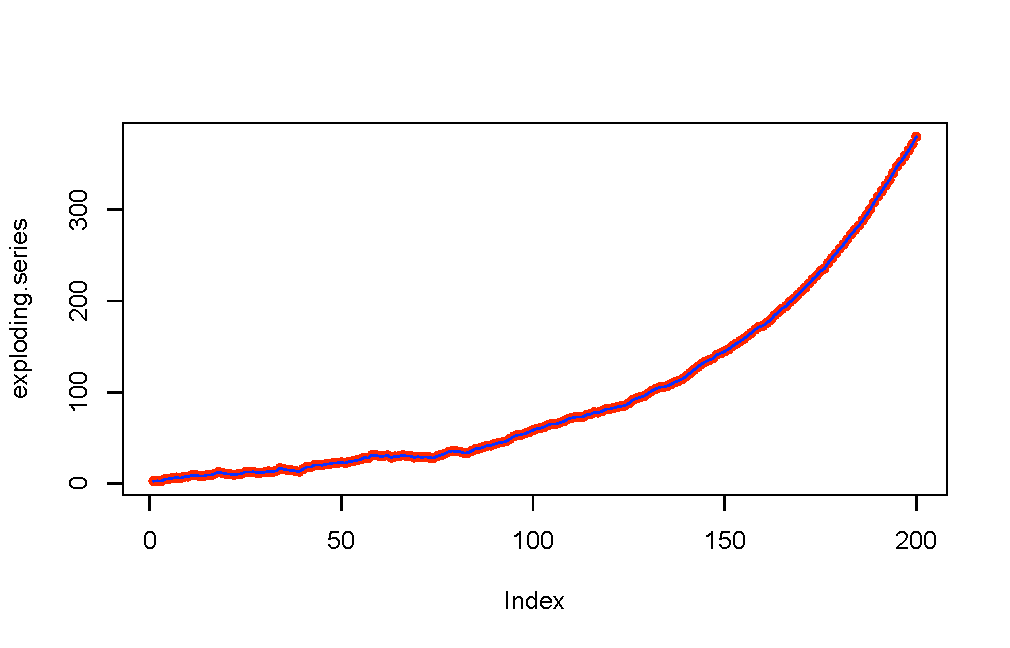
\includegraphics[width=4in]{../graphs/exploding}
\vskip -.3cm
\small
Since the series explodes, it is useless for modeling and prediction.
\end{frame}



\begin{frame}

{\bf Stationary Series}\sk

\small For AR term $<1$, $Y_t$ is always pulled back towards the mean.

\begin{center}
$\beta_1 = 0.8$
\end{center}
\vskip -1.5cm
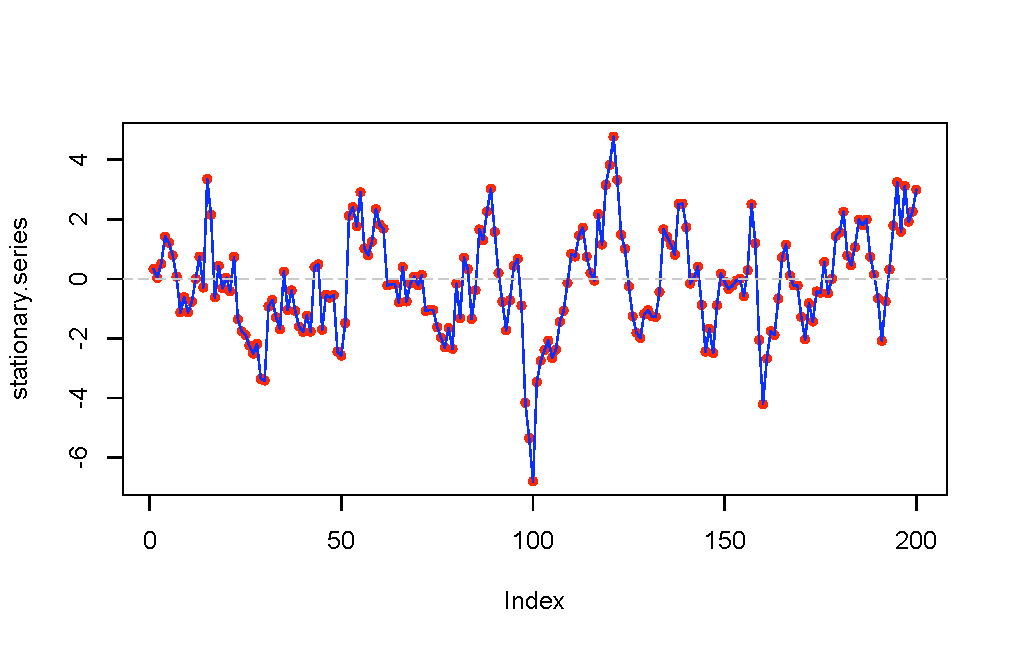
\includegraphics[width=4in]{../graphs/stationary}
\vskip -.3cm
\small
These are the most common, and most useful, type of AR series.

\end{frame}


\begin{frame}

{\bf Stationary Series}\sk

Autocorrelation for the stationary series drops off right away.

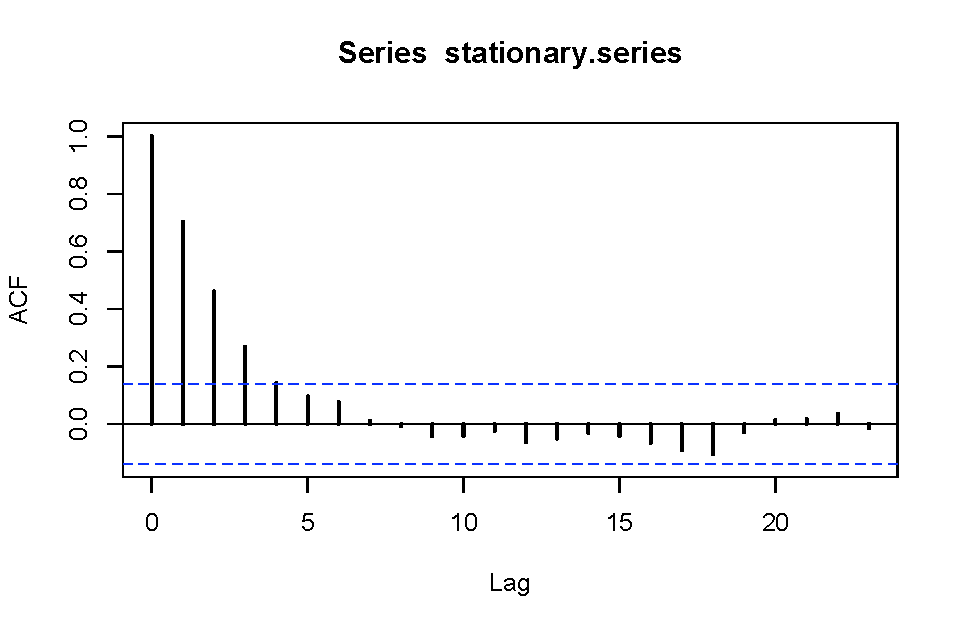
\includegraphics[width=4in]{../graphs/acfstationary}
\vskip -.3cm
\small
The past matters, but with limited horizon.

\end{frame}


\begin{frame}

{\bf Mean Reversion}\sk

An important properties of stationary series is \theme
mean reversion\bk.

\sk
Think about shifting both $Y_t$ and $Y_{t-1}$ by their mean $\mu$.
\[ \nv Y_t - \mu = \beta_1 (Y_{t-1} - \mu) +\varepsilon_t
\]
Since $|\beta_1| < 1$, $Y_t$ is expected to be closer to the $\mu$
than $Y_{t-1}$.

\sk 
Mean reversion is all over, and helps  predict
future behaviour.
\begin{itemize}
\item  ``alpha'' in repeated CAPM models.
\item  Weekly sales numbers.
\item  Daily temperature.
\end{itemize}

\end{frame}



\begin{frame}

{\bf Negative Correlation}\sk

It is also possible to have negatively correlated AR(1) series,
but you see these far less often in practice.

\begin{center} \vskip -.1cm
$\beta_1 = -0.8$
\end{center}
\vskip -1.5cm
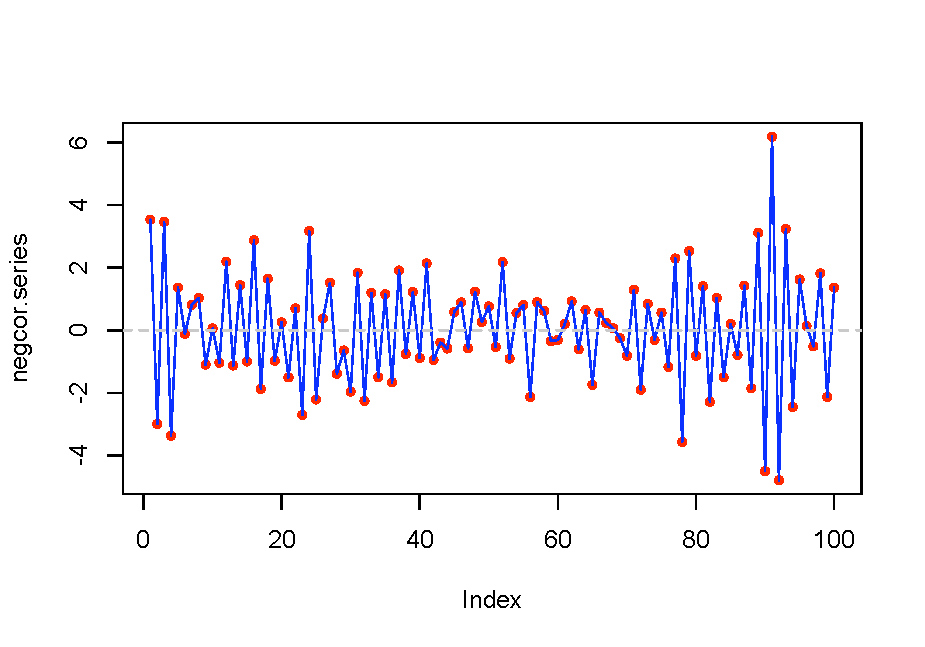
\includegraphics[width=4in]{../graphs/negcor}
\end{frame}

\begin{frame}

{\bf Summary of AR(1) Behavior}\sk

\small
\begin{itemize}
\item [$|\beta_1| < 1$]
The series has a mean level to which it reverts.  For 
positive $\beta_1$, the series tends to wander above or below 
the mean level for a while.  For negative $\beta_1$, the series 
tends to flip back and forth around the mean. 
The series is stationary, meaning that the 
mean level does not change over time.  
\item [$|\beta_1| = 1$] A random walk series.
The series has no mean level and, thus, is called 
nonstationary.  The drift parameter $\beta_0$ is the direction in 
which the series wanders.
\item [$|\beta_1| > 1$] 
The series explodes, is nonstationary, and pretty much useless.
\end{itemize}
\end{frame}


\begin{frame}

{\bf AR(p) Models}\sk

It is possible to expand the AR idea to higher lags
\[
\nv AR(p): Y_t = \beta_0 + \beta_1Y_{t-1} + \ldots \beta_pY_{t-p} + \varepsilon
\]
\vskip -.5cm
Drawback: you lose the stationary/nonstationary
intuition.

\vskip .25cm
And often the need for higher lags is symptomatic of your missing a more
persistent trend or periodicity in the data.

\vskip .25cm
Previous classes probably warned against using $p>1$.

\vskip .25cm
However: with lasso at your disposal, I'm OK with you just throwing in higher lags and letting it choose what you need. \\{\theme  Datamine the lags!}

\end{frame}

\begin{frame}

{\bf Spatial extensions}

\sk Space is just like time, but with another dimensions!


\vskip .25cm

To include dependence, you again include $y_{\bm{s}}$ for other $\bm{s}$.

\vskip .25cm
For example, in your regression you can include

\vskip .2cm ~~~~~~~~~~~~ $\bullet$ the average for neighboring states.

\vskip .2cm ~~~~~~~~~~~~ $\bullet$ the average of the neighboring pixels.

\sk
There are a ton of more compicated routines for when modeling temporal or 
spatial effects is your primary interest. {\gr gaussian processes, kriging,
state-space models, GARCH, etc...}

{\theme Another time in another class!}


\end{frame}



\end{document}
